% !TEX root = seminararbeit.tex

\section{Prelude}
\label{sec:Prelude}

The goal of the thesis is to create a 3D editor, using web technologies,
which enables its users to postprocess x3d scenes. These scenes are the
result of a tool which was implemented as part of the DFG research
project Roundtrip3D. The scene are automatically derived from
software models \ldots{}

\subsection{Motivation}\label{motivation}

As part of the Roundtrip3D project, a round-trip framework (hereafter
referred to as \emph{R3D}) was developed. This framework also includes a
graphical editor for SSIML models, to describe 3D applications. Then the
R3D can be used to generate boilerplate code for multiple programming
languages, such as JavaScript, Java or C++, and an X3D file describing
the scene. The X3D file may contain references to other X3D files
containing the actual 3D data (e.g.~a car and the corresponding tires),
hereafter called \emph{inlines} . These files are created by exporting
objects from a 3D computer graphics software (e.g. Blender,
Maya or 3DS Max).\\
The problem that arises is that each object is usually in the center of
it's own coordinate system. So they need to be translated, rotated and
maybe even scaled to result in desired scene (e.g.~a car where the tires
are in the places they belong to and not in the center of the chassis).
The structure is mostly generated. Attribute values of respective nodes,
such as transformation nodes need to be adjusted in order to compose the
overall 3D scene.

% \includegraphics{Picture of a car with the tires in the center}\\
% \includegraphics{Picture of a car with the tires where they belong to}

This can be achieved by adjusting \emph{translate}, \emph{rotate} and
\emph{scale} properties to arrange 3D objects. To exacerbate this
problem further, the orientation the 3D artists chose for it's object is
simply unknown, if their is no convention for 3D modeling. \sout{Usually
their is a convention about origin of coord system, scaling and
orientation} (no there isn't, still not sure what to put here). However, we cannot assume that these
conventions are always met. The main problem is, that 3D
transformations, such as translation, orientation and scale of single 3D
geometries, need to be adjusted. So far, there is no graphical tool that
meets both of these requirements:

\begin{itemize*}
\item user friendly and straight forward compose functionalities of X3D scenes
\item and preservation of (generated) information, such as node names or comments (necessary to merge the changed files back into the source model)
\end{itemize*}

The figures \ref{fig:wheel1} - \ref{fig:wheel4} demonstrate the problem.

\begin{figure}[htbp]
  \begin{minipage}{.5\textwidth}
    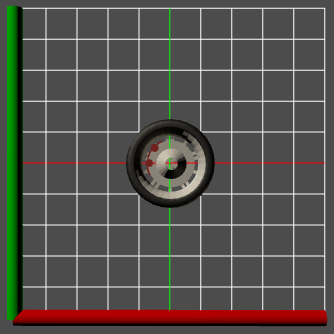
\includegraphics[width=0.9\textwidth]{../assets/wheel1.png}
  	\caption{Wheel 1}
  	\label{fig:wheel1}
  \end{minipage}
  \begin{minipage}{.5\textwidth}
  	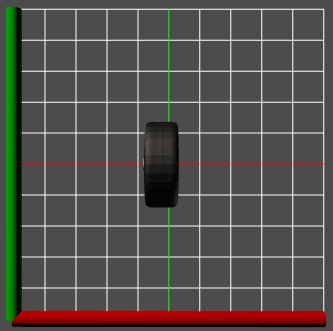
\includegraphics[width=0.9\textwidth]{../assets/wheel2.png}
  	\caption{Wheel 2}
  	\label{fig:wheel2}
  \end{minipage}\\
  \begin{minipage}{.5\textwidth}
  	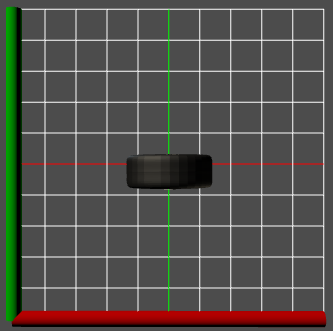
\includegraphics[width=0.9\textwidth]{../assets/wheel3.png}
  	\caption{Wheel 3}
  	\label{fig:wheel3}
  \end{minipage}
  \begin{minipage}{.5\textwidth}
  	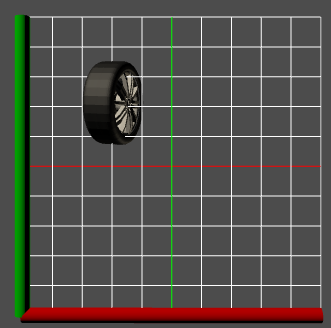
\includegraphics[width=0.9\textwidth]{../assets/wheel4.png}
  	\caption{Wheel 4}
  	\label{fig:wheel4}
  \end{minipage}
\end{figure}

\ref{fig:wheel1} to \ref{fig:wheel3} are common orientations, since it's disputable which of these
could be considered be the norm.\\
But if one depends on art from 3rd parties, the orientation and position
could be completely arbitrary like in figure \ref{fig:wheel4}\\

These properties could be added and adjusted via any text editor by
opening the generated x3d file, but the resulting workflow isn't
user-friendly:

\begin{enumerate*}
  \item model 3D application, including 3D scene structure
  \item generate 3D scene and application code
  \item run application and evaluate the scene and think about what objects need to go where and whether they need to be scaled
  \item type random translation, rotation and scale
  \item run the application again and evaluate whether the transformations is correct (since one does not know anything about the orientation of the object)
  \item go back to 4. until all objects are placed correctly
\end{enumerate*}

Tools like Maya or Blender could also be used for this, but their import
and export filter discard important metadata that is necessary for the
round-trip transformation. This is what SceGraToo is meant to be.

SceGraToo addresses both of these issues. It allows for loading the root
X3D file and changing all transformations, containing the inline nodes,
using mouse interactions. For fine grained control SceGraToo also
contains a tree view that allows the user to input exact attributes for
translations, rotations and scale.

\subsection{Scope}\label{scope}

This thesis addresses two issues:

\begin{enumerate*}
  \item allowing for composing generated X3D scenes (with focus on usability). E. g., besides a 3D view, a tree view for fine grained editing should not only visualize the 3D scene's structure, but also allow for entering concrete coordinate values.
  \item during the editing process, the preservation of all information/metadata must be guaranteed.
\end{enumerate*}
